% Institute of Computer Science thesis template
% authors: Sven Laur, Liina Kamm
% last change Tõnu Tamme 09.05.2017
%--
% Compilation instructions:
% 1. Choose main language on line 55-56 (English or Estonian)
% 2. Compile 1-3 times to get refences right
% pdflatex bachelors-thesis-template
% bibtex bachelors-thesis-template
%--
% Please use references like this:
% <text> <non-breaking-space> <cite/ref-command> <punctuation>
% This is an example~\cite{example}.

\documentclass[12pt]{article}

% A package for setting layout and margins for your thesis 
\usepackage[a4paper,marginparsep=10pt,marginparwidth=80pt]{geometry}
%TODO: margin has been modified

%%=== A4 page setup ===
%\setlength{\paperwidth}{21.0cm} 
%\setlength{\paperheight}{29.7cm}
%\setlength{\textwidth}{16cm}
%\setlength{\textheight}{25cm}


% When you write in Estonian then you want to use text with right character set
% By default LaTeX does not know what to do with õäöu letters. You have to specify
% a correct input and font encoding. For that you have to Google the Web     
%
% For TexShop under MacOS X. The right lines are 
%\usepackage[applemac]{inputenc}
%\usepackage[T1]{fontenc} %Absolutely critical for *hyphenation* of words with non-ASCII letters.
%
% For Windows and Linux the right magic lines are   
% \usepackage[latin1]{inputenc}
% \usepackage[latin5]{inputenc}
%%\usepackage[utf8]{inputenc} %Package inputenc Error: Unicode char ´ (U+B4) not set up for use with LaTeX
\usepackage[utf8x]{inputenc}
\usepackage[T1]{fontenc} %Absolutely critical for *hyphenation* of words with non-ASCII letters.

% Typeset text in Times Roman instead of Computer Modern (EC)
\usepackage{times}

% Suggested packages:
\usepackage{microtype}  %towards typographic perfection...
\usepackage{inconsolata} %nicer font for code listings. (Use \ttfamily for lstinline bastype)
\usepackage[parfill]{parskip} %no indents, empty lines instead


% Use package babel for English or Estonian 
% If you use Estonian make sure that Estonian hyphenation is installed 
% - hypen-estonian or eehyp packages
%
%===Choose the main language in thesis
\usepackage[estonian, english]{babel} %the thesis is in English 
%\usepackage[english, estonian]{babel} %the thesis is in Estonian


% Change Babel document elements 
\addto\captionsestonian{%
  \renewcommand{\refname}{Viidatud kirjandus}%
  \renewcommand{\appendixname}{Lisad}%
}


\usepackage{natbib}
\renewcommand{\cite}{\citep}
\usepackage{apalike}
\bibliographystyle{apalike}


% General packages for math in general, theorems and symbols 
% Read ftp://ftp.ams.org/ams/doc/amsmath/short-math-guide.pdf for further information
\usepackage{amsmath} 
\usepackage{amsthm}
\usepackage{amssymb}

% Optional calligraphic fonts    
\usepackage[mathscr]{eucal}

% Print a dot instead of colon in table or figure captions
\usepackage[labelsep=period]{caption}

% Packages for building tables and tabulars 
\usepackage{array}
\usepackage{tabu}   % Wide lines in tables
\usepackage{xspace} % Non-eatable spaces in macros

% Including graphical images and setting the figure directory
\usepackage{graphicx}
\graphicspath{{figures/}}

% Packages for getting clickable links in PDF file
%\usepackage{hyperref}
\usepackage[hidelinks]{hyperref} %hide red (blue,green) boxes around links
\usepackage[all]{hypcap}

\usepackage{url}

\usepackage[acronym,toc,numberedsection,automake]{glossaries}
\makeglossaries
\newacronym{obc}{OBC}{On-Board Computer}
\newacronym{mcu}{MCU}{Microcontroller Unit}
\newacronym{cdhs}{CDHS}{Command and Data Handling System}
\newacronym{com}{COM}{Communication System}
\newacronym{crc}{CRC}{Cyclic Redundancy Check}
\newacronym{eeprom}{EEPROM}{Electrically Erasable Programmable Read-Only Memory}
\newacronym{eps}{EPS}{Electrical Power System}
\newacronym{eseo}{ESEO}{European student Earth orbiter}
\newacronym{fram}{FRAM}{Ferroelectric Random Access Memory}
\newacronym{i2c}{I2C}{Interintegrated Circuit}
\newacronym{icp}{ICP}{Internal Communications Protocol}
\newacronym{mmu}{MMU}{Memory Management Unit}
\newacronym{elf}{ELF}{Executable and Linkable Format}
\newacronym{got}{GOT}{Global Offset Table}
\newacronym{fpga}{FPGA}{Field-Programmable Gate Array}


\usepackage[titletoc,title,page]{appendix}

% Packages for defining colourful text together with some colours
\usepackage{color}
\usepackage{xcolor} 
%\definecolor{dkgreen}{rgb}{0,0.6,0}
%\definecolor{gray}{rgb}{0.5,0.5,0.5}
\definecolor{mauve}{rgb}{0.58,0,0.82}


% Standard package for drawing algorithms
% Since the thesis in article format we must define \chapter for
% the package algorithm2e (otherwise obscure errors occur) 
\let\chapter\section
\usepackage[ruled, vlined, linesnumbered]{algorithm2e}

% Fix a  set of keywords which you use inside algorithms
\SetKw{True}{true}
\SetKw{False}{false}
\SetKwData{typeInt}{Int}
\SetKwData{typeRat}{Rat}
\SetKwData{Defined}{Defined}
\SetKwFunction{parseStatement}{parseStatement}


% Nice todo notes
\usepackage[prependcaption]{todonotes}

% comments and verbatim text (code)
\usepackage{verbatim}


% Proper way to create coloured code listings
\usepackage{listings}
\lstset{ 
  %language=python,                % the language of the code
  language=C,
  basicstyle=\footnotesize,        % the size of the fonts that are used for the code
  %numbers=left,                   % where to put the line-numbers
  %numberstyle=\footnotesize,      % the size of the fonts that are used for the line-numbers
  numberstyle=\tiny\color{gray}, 
  stepnumber=1,                    % the step between two line-numbers. If it's 1, each line 
                                   % will be numbered
  numbersep=5pt,                   % how far the line-numbers are from the code
  backgroundcolor=\color{white},   % choose the background color. You must add \usepackage{color}
  showspaces=false,                % show spaces adding particular underscores
  showstringspaces=false,          % underline spaces within strings
  showtabs=false,                  % show tabs within strings adding particular underscores
  frame = lines,
  %frame=single,                   % adds a frame around the code
  rulecolor=\color{black},		   % if not set, the frame-color may be changed on line-breaks within 
                                   % not-black text (e.g. commens (green here))
  tabsize=2,                       % sets default tabsize to 2 spaces
  captionpos=b,                    % sets the caption-position to bottom
  breaklines=true,                 % sets automatic line breaking
  breakatwhitespace=false,         % sets if automatic breaks should only happen at whitespace
  %title=\lstname,                 % show the filename of files included with \lstinputlisting;
                                   % also try caption instead of title
  keywordstyle=\color{blue},       % keyword style
  commentstyle=\color{dkgreen},    % comment style
  stringstyle=\color{mauve},       % string literal style
  escapeinside={\%*}{*)},          % if you want to add a comment within your code
  morekeywords={*,game, fun}       % if you want to add more keywords to the set
}


% Obscure packages to write logic formulae and program semantics
% Unless you do a bachelor thesis on program semantics or static code analysis you do not need that
% http://logicmatters.net/resources/ndexamples/proofsty3.html <= writing type rules => use semantic::inference
% ftp://tug.ctan.org/tex-archive/macros/latex/contrib/semantic/semantic.pdf
% \usepackage{proof}
% \usepackage{semantic} 
% \setlength{\inferLineSkip}{4pt}
% \def\predicatebegin #1\predicateend{$\Gamma \vdash #1$}

% If you really want to draw figures in LaTeX use packages tikz or pstricks
% However, getting a corresponding illustrations is really painful  


% Define your favorite macros that you use inside the thesis 
% Name followed by non-removable space
\newcommand{\proveit}{ProveIt\xspace}

% Macros that make sure that the math mode is set
\newcommand{\typeF}[1] {\ensuremath{\mathsf{type_{#1}}}\xspace}
\newcommand{\opDiv}{\ensuremath{\backslash \mathsf{div}}\xspace} 

% Nice Todo box
\newcommand{\TODO}{\todo[inline]}

% A way to define theorems and lemmata
\newtheorem{theorem}{Theorem}


\input{variables_README.tex}
\input{variables_LOEMIND.tex}

\newcommand{\topic}{\iflanguage{english}{\Title}{\Pealkiri}}


%%% BEGIN DOCUMENT
\begin{document}

% Title page
%===BEGIN TITLE PAGE
\thispagestyle{empty}
\begin{center}

\iflanguage{english}{%
\large
UNIVERSITY OF TARTU\\%[2mm]
Institute of Computer Science\\
Computer Science Curriculum\\%[2mm]
}{%
TARTU ÜLIKOOL\\
Arvutiteaduse instituut\\
Informaatika õppekava\\%[2mm]
}%\iflanguage

%\vspace*{\stretch{5}}
\vspace{25mm}


\Large \Author
\vspace{4mm}

\huge\topic

%\vspace*{\stretch{7}}
\vspace{20mm}

\iflanguage{english}{%
\Large Bachelor's Thesis (9 ECTS)
}{%
\Large Bakalaureusetöö (9 EAP)
}%\iflanguage

\end{center}

\vspace{2mm}

\begin{flushright}
 {
 \setlength{\extrarowheight}{5pt}
 \begin{tabular}{r l}
  \sffamily \iflanguage{english}{Supervisor}{Juhendaja}: & \sffamily \SupervisorTitlepage \\
  \sffamily \iflanguage{english}{Supervisor}{Juhendaja}: & \sffamily \CosupervisorTitlepage
 \end{tabular}
 }
\end{flushright}

%\vspace*{\stretch{3}}
%\vspace{10mm}

\vfill
\centerline{Tartu 2018}

%===END TITLE PAGE


% If the thesis is printed on both sides of the page then 
% the second page must be must be empty. Comment this out
% if you print only to one side of the page comment this out
%\newpage
%\thispagestyle{empty}    
%\phantom{Text to fill the page}
% end of extra page without number

% Information page
%===COMPULSORY INFO PAGE
\newpage

%=== Info in English
\newcommand\EngInfo{{%
\selectlanguage{english}
\noindent\textbf{\large\topic}

\vspace*{3ex}

\noindent\textbf{Abstract:}

\noindent\Abstract

\vspace*{1ex}

\noindent\textbf{Keywords:}\\ \Keywords

\vspace*{1ex}

\noindent\textbf{CERCS:} \CERCS

\vspace*{1ex}
}}%\newcommand\EngInfo

%=== Info in Estonian
\newcommand\EstInfo{{%
\selectlanguage{estonian}
\noindent\textbf{\large \topic}
\vspace*{3ex}

\noindent\textbf{Lühikokkuvõte:} 

\noindent\Abstrakt

\vspace*{1ex}

\noindent\textbf{Võtmesõnad:}\\ \Mrksnad

\vspace*{1ex}

\noindent\textbf{CERCS:} \Teaduseriala

\vspace*{1ex}
}}%\newcommand\EstInfo


%=== Determine the order of languages on Info page
\iflanguage{english}{\EngInfo}{\EstInfo}
\newpage
\iflanguage{estonian}{\EngInfo}{\EstInfo}


% Table of contents
\newpage
\tableofcontents

% Remember to remove this from the final thesis version
\newpage
\TODO{Remove list of todos}
\listoftodos[Unsolved issues]
% end of todo page 


%%% Content
\newpage
\section{Introduction}

Main goal of this thesis is to design and implement a method of updating software more suitable for ESTCube-2 than existing alternatives. Proposed solution focuses on enabling delta updates (avoiding upload of unchanged code as much as possible) and reducing the amount of on-board processing required. Additionally, updatable software's performance nor abilities should be limited either.

During the ESTCube-2 mission, loading of new software onto the satellite is planned, in order to introduce new features, test and compare novel software solutions, and resolve potential software or hardware issues. The value of increased software flexibility is measurable and can be higher than, for example, that of hardware flexibility \cite{Nilchiani2009}. For updating software on ESTCube-2, main difficulties are slow uplink (9600 bits per second), limited on-board processing power \cite{Ehrpais2016}, execution of software from Flash memory \cite{Haljaste2017} (limitations of which are detailed in Section~\ref{s:hardware}), and frequent updates due to the missions experimental nature.

All existing solutions for updating software have limitations (described in Section~\ref{s:relatedwork}) when applied to the \gls{obc} of ESTCube-2. The topic is relevant right now, since ESTCube-2 is currently in development phase. Even though this thesis focuses on the use cases of ESTCube-2, the topic has wider importance - several existing solutions have been designed with Internet of Things or wireless sensor networks \cite{Dunkels2006,Han2005} in mind. Those systems have several common aspects with nanosatellites. The method proposed in this thesis has not been previously described in literature.

Scope of this work is limited to on-board software written in C, GNU toolchain, and standard FreeRTOS distribution.

\subsection{ESTCube-2}

ESTCube-2 is an experimental three-unit CubeSat. The mission is planned to serve as an in-orbit demonstration of the platform, which could then be employed on future missions. \cite{Iakubivskyi2016}

\textcite{Iakubivskyi2016} list among the systems to be tested on ESTCube-2
\begin{itemize}
  \item tether module for plasma brake deorbiting (previous versions of which have flown on the satellites ESTCube-1 and Aalto-1)
  \item Earth observation camera system (which is based on the \gls{eseo} camera)
  \item high speed C-band downlink system
  \item a novel miniaturized (up to 0.6 units) satellite bus
  \item cold gas propulsion module by NanoSpace,
  \item thin film protective coating experiment by Captain Corrosion OÜ.
\end{itemize}


ESTCube-2 is developed mostly by the students of University of Tartu and students that join the ESTCube program from all over the world \cite{Ehrpais2016}. Also among the main objectives for ESTCube-2 is to educate a new generation of space engineers, and to promote space technologies in general \cite{Iakubivskyi2016}.

The \gls{obc} of the satellite is tasked with running \gls{aocs} algorithms, controlling payload experiments and star tracker, and handling telemetry and telecommands. The most important requirements for \gls{aocs} are set by plasma brake and Earth observation payloads. The former needs sufficient enough angular momentum for the centrifugal deployment of the tether, and the latter requires accurate pointing. While some methods, like the use of magnetic torquers, build upon the heritage of the successful ESTCube-1 mission, others, like reaction wheels by Hyperion Technologies and in-house developed star tracker, are completely new for the team. Due to the large amount of experimental software, it is planned that it should be possible to perform firmware updates on all of the \glspl{mcu} after the launch of the satellite. This enables the team to correct any unexpected problems that the satellite may encounter. \cite{Ehrpais2016}


\subsection{Outcomes}

Primary difficulty tackled in this thesis is how to add new or updated functions incrementally without the need for on-board modifications. Taking into account that and the scope of this thesis, main subject of research is how GNU C compiler generates machine code, and what are the options to alter the process to suit specific needs. Modifying the compiler itself is outside of the scope of this thesis, but in addition to compiler configuration flags, pre- and post-processing are utilized.

The method proposed in this thesis considers a function to be an atomic unit. Functions would be compiled separately and only new or updated functions would be uploaded.  This way less data needs to be uploaded while preserving software's native performance and abilities. Received functions would be stored sequentially in Flash memory without modifications. The need to delete Flash memory for each update is eliminated, making it possible to add new functions even without rebooting the embedded system. Performance, applicability and limitations of proposed solution are analyzed.

The rest of this thesis is organized as follows. Section~\ref{s:usecases} lists use cases based on ESTCube-1 experience and planned ESTCube-2 hardware. Section~\ref{s:relatedwork} describes identified four categories of previous approaches to the problem of embedded software updates. Strengths and weaknesses of them are listed. Section~\ref{s:design} describes the solution proposed in this thesis along with detailed requirements. Section~\ref{s:testing} includes results of testing the solution. Appendix~\ref{acronym} lists all used abbreviations. Appendix~\ref{apx:calls} has an experiment that explains, why function table was implemented with four bytes per function. Appendix~\ref{apx:gentable} includes the bootloading procedure needed to make proposed solution work. Appendix~\ref{apx:cos} demonstrates an example of a very short function from an in-development \gls{aocs} library.

\newpage
\section{Use cases}
\label{s:usecases}

Use cases for the ESTCube-2 \gls{obc} software updating system (predictions on how the system will need to be used later on) are derived from ESTCube-1 \gls{cdhs} experience. Differences between the two missions are taken into account where applicable.

\subsection{ESTCube-1 experience}

ESTCube-1 \gls{cdhs} received 20 distinct firmware updates during its mission, with 19 of them being successful \cite{Suenter2016}. \textcite{Slavinskis2015} list among functionalities added to the \gls{cdhs} ``power saving mode, variety of data logging functions, high time-resolution functions for sensor measurements, experiment-related functions, additional preprocessing of attitude measurements, as well as attitude determination and control algorithms.'' Some of the changes were introduced in response to unforeseen circumstances.

Size of the changes in corresponding source codes was analyzed. On average, 2.09\% ($\sigma$=3.43\%) of the code lines were added, removed or edited during a firmware update. The largest update changed 14.71\% of the code, while the smallest update only modified 0.02\% of all the lines. Updates with largest code changes were so due to addition of large portions of new code. Overall, size of the source code for \gls{cdhs} software (including all libraries) also gradually increased through the mission (from 63~390 lines of code to 78~868, a 24.42\% increase). However, no update consisted of just new code being added, always some previously existing code was changed or removed as well.

As it was on ESTCube-1 (a classic nonsegmented firmware), a minor code modification could result in a binary difference of almost 99\%, which caused the need to upload an entire firmware image again every time. Size of a typical \gls{cdhs} firmware image after compilation was 250 kibibytes. Those images had a Shannon entropy of about 0.6 (on the scale of 0$-$1), resulting in a theoretical maximum compression ratio of 40\%. \cite{Suenter2016}

\subsection{Use cases during ESTCube-2 mission}

The hardware, on which the software will be updated, significantly affects the choice of updating method. This choice is also dependent on the properties of the updates themselves, which can differ notably due to different reasons causing the need for those updates.

\subsubsection{ESTCube-2 hardware}\label{s:hardware}

ESTCube-2 \gls{obc} will be centered around an STM32F767IIT6 \gls{mcu}, which has 2 mebibytes\footnotemark of internal flash and 516 kibibytes\footnotemark[\value{footnote}] of internal \gls{sram}. For the data of running programs the \gls{obc} has 2 mebibytes\footnotemark[\value{footnote}] of \gls{mram}. For external configuration tables, error logs, on-board statistics, and other data without strict latency restrictions, it has 3$\times$512 kibibytes\footnotemark[\value{footnote}] of \gls{fram}. Mass storage for firmware versions, measurements, and payload data is provided by 2$\times$32 mebibytes\footnotemark[\value{footnote}] of external flash.
\cite{Haljaste2017}

At least critical software components must be stored in the internal flash, so that it would be possible to disable all external device drivers in safe mode. This is desirable since having more code enabled increases the probability of any faults occurring. However, flash memory consists of sectors, which can be up to 256 kibibytes\footnotemark[\value{footnote}] in size \cite{STMicroelectronics2018}. In order to edit any data already written to the memory, an entire sector must be erased and rewritten \cite{STMicroelectronics2018}.

\footnotetext{\label{fn:units}Cited sources claim those numbers to be in decimal units (kilo- and megabytes), but are assumed to do so by mistake.}

\subsubsection{Types of updates}

Due to the limited number of suitable launches (caused mostly by limited funding possibilities), it might happen that the satellite has to be delivered on an unexpectedly accelerated schedule, so that some software functionalities are not completed or sufficiently tested before the launch. In such case, significant amounts of new code would need to be added to the firmware with an update. Additionally, some previous code would need to be modified to make use of those new functionalities. However, largest parts of the firmware by size - \gls{os}, \gls{hal} and drivers - must definitely be finalized before the launch in order to enable successful satellite operation. This means that the size of even the largest update caused by this reason would stay under about 20\%.

Several software components are experimental. In order to assess the properties of novel solutions, they need to be compared with existing methods, which could mean the need to deploy alternative algorithms for some period of time. However, swapping out a software component could not cause changes larger than introducing a new feature.

The testing of novel software solutions also entails the need for iterative improvements, as the perfect setup is unlikely to be achieved on the first try. While most of this should be possible by only changing configuration values separate from the firmware, it might happen that some unforeseen change does require code rewriting. Updates for aforementioned reasons would affect only a small number of components and would alter significantly less than 1\% of the firmware.

When bugs are discovered in on-board software, a fix needs to be developed and deployed. Such update would mostly consist of changes to the existing code, and can be expected to change considerably less than 1\% of the firmware. Changes would also be limited to a single component or functionality. When a bug is discovered, it may be necessary to deploy the fix without delays, to minimize the probability of any mission critical risks materializing.

Unforeseen issues are also possible with the satellite hardware, due to the use of \gls{cots} components, extreme miniaturization, and the educational nature of the development process. Some of such issues could be circumvented with software workarounds. These can range from simple code changes to the addition of completely new functionality.

Lastly, the main mission of ESTCube-2 is to conduct experiments, like unreeling the plasma brake tether. During experiments it might be useful to rapidly deploy new small subroutines that handle aspects of the experiment that were not predicted beforehand.

\newpage
\section{Related work}

The problem of software updates on embedded systems has seen many different solutions so far. A brief overview of existing methods is given in this section.

\subsection{Full system image replacement}

% generic overview of what the method is (+ estcube-1)
For example, on ESTCube-1, one of the ways to update on-board code was to recompile the entire code-base, including any changes, upload it to the satellite, and after the next reboot of the \gls{mcu}, this new code would be active \cite{Suenter2016}. This method benefits from a rather simple design: compilation of complete system image is typically the default way to produce executables with embedded operating systems from day zero of development \todo{citation?}. Additionally, by replacing the entire system image, any interoperability issues are eliminated and next to none on-board processing is required. Support for full image replacement is often implemented as fallback even on systems that support other more advanced update mechanisms as well \cite{Tarbe2013,Greco2005,Garrido1998}.

% dual images
Additionally, several missions have had the ability to keep several such system images stored at any time, allowing switching between them in case of any unexpected problems. In some cases, like MINISAT01, one of the images was read-only and only other one could be modified \cite{Garrido1998}. However, in some other cases, like  ESTCube-1 \cite{Tarbe2013} and The Mars Exploration Rovers \cite{Greco2005}, it has been possible to update both firmware images independently. The former poses significant drawbacks: in the case of MINISAT01, complete firmware update took 2 full days, and for that duration the original launch firmware version had to be used \cite{Garrido1998}. 

\TODO{Few words about bootloaders on ESTCube-1 and Mars Exploration Rovers.}

% drawbacks + estcube-1
However, this kind of simple design also poses significant drawbacks. Most importantly, it requires large amounts of uplink, even if the change was minor. For example, on ESTCube-1, taking into account the size of the firmware, uplink speed and orbital parameters, uninterrupted firmware update would take about 1.5 days to complete \cite{Suenter2014}. In case of the MINISAT01, full firmware update took 2 complete days, while partial update could be done in few hours \cite{Garrido1998}. In case of The Mars Exploration Rovers, replacement of entire firmware image required uplinking 8 Megabytes of data, while a patch update that they completed only required the uplinking of approximately 2 Megabytes \cite{Greco2005}.

\subsection{Virtual machines and script interpreters}

Another method that is commonly used when new code needs to be uploaded frequently and in small parts, is utilize visualization techniques on board. For example interpreted scripting language pawn script was used on ESTCube-1 \cite{Suenter2016} and will be used on TTÜ100 satellite \cite{Aasavaeli2017}. With this approach some parts of the code are written in native code and some as scripts. Since scripts only interact with rest of the system through previously defined API-s, they can be modified without influencing any other parts of the system. Thanks to the abstraction layer that the script interpreter provides, script files can be moved and rearranged without difficulty \cite{Riemersm}.

However, not all of the on-board software can be rewritten this way. Script execution is significantly slower than the that of a native code \todo{script vs native speed comparison}. Additionally, scripts have limited access to other system resources through predefined API-s.

\TODO{About actual virtual machines}

\subsection{Binary differences}

In order to overcome the large uplink requirements of full image replacement while keeping the benefits of native code, some authors have experimented with calculating a delta between two system images and using it to recreate new image on-board.

One of the simplest binary difference based approaches for delta software updates was implemented on MINISAT01. Their entire firmware image consisted of 32 parts, and they could be updated separately. While updating the whole firmware took two full days, updating a single part could be done in just few hours. However, this approach had a serious limitation: old and updated codes had to be exactly binary compatible, no lengths could be changed. Therefore this kind of approach is only useful for updating values of constants, since code updates typically also change the length of compiled binary. \cite{Garrido1998}

To overcome this limitation, MINISAT01 also featured third method of updating on-board software. With this method, new or updated functions were located at the end of the firmware, while old versions were kept on their original locations. Then any calls to modified functions were changed in on-board software. This was possible, since modifying function call with new location does not change the length of the call, and MINISAT01 stored its firmware in \gls{eeprom}. \cite{Garrido1998} \todo{what is Global Description Table?}

A more complex approach to binary difference based software updates was taken on The Mars Exploration Rovers. They calculated differences between new and old firmware images that could start and end at arbitrary locations and change image size as well. However, to achieve this, they had to build the updated image in volatile memory and then store generated updated image in non-volatile memory. This meant that they had to reserve full day to assemble, validate and store the updated software. During that time no other activities could be carried out. They also acknowledge that "The single biggest improvement to the Mars Explorer Rovers' flight software modification process would be to reduce the amount of time necessary to stand down from nominal surface operations." \cite{Greco2005}

\subsection{Dynamically loaded modules}

Early solutions in desktop operating systems for loading new software programs without changing the entire system used hardware \gls{mmu} to provide virtual separate memory space for each component \todo{citation (PIC) required}. This way code could be statically linked without conflicts. Embedded systems that have an \gls{mmu}, have similarly used server-side pre-linking of software \cite{Shen2010}.

A very similar problem to that of embedded systems without an \gls{mmu} has been solved on desktop for shared libraries. While on embedded systems code modifications are undesirable due to limited computational power and the use of Flash memory, on desktop systems code modifications would force several versions of the same library to be kept in memory. Neither can be statically linked in order to avoid conflicts between different modules. The solution is to compile software in a position independent manner by introducing some sort of jump table for indirection \todo{citation for PIC required}. Hybrid solutions of pre-linking and pre-locating combined with dynamic re-location have also been explored \cite{Dong2009}. 

The jump table can be part of the operating system memory or part of each module. Example of the former can be found in the SOS operating system, where each module has to register functions into the jump table \cite{Han2005}. The latter approach has been implemented in, for example, Contiki OS, that makes use of modified \gls{elf} to hold code alongside its \gls{got} \cite{Dunkels2006}. Unfortunately, dynamic linking of \gls{elf} files is still not widely supported on embedded operating systems \cite{Xinyu2017}. Among others like it, FreeRTOS (the operating system used on ESTCube-2 \gls{obc}) does not support loading modules dynamically \cite{Barry2005}. \citet{Xinyu2017} describes a method for including the code relocation functionality into the relocatable code itself as one possible solution.



\newpage
\section{Design approach}
\label{s:design}

As shown, no existing solution fully covers the described use cases, and this mandates further research. This section defines requirements for a system that would be more suitable for ESTCube-2 than any existing alternatives. Possible design for meeting those requirements is also proposed.

\subsection{Requirements}

Software updating system that would be more suitable for ESTCube-2 than any existing alternatives, must:

\begin{enumerate}
	\item allow addition of program code without the need to re-transmit significant portions of already existing code, so that it could be used for small one-time subroutines as well.
	\item allow changing a subset of existing code without the need to re-transmit significant portions of unchanged code, so that upload bandwidth and update application time would be minimized.
	\item not require on-board modifications of uploaded code. This makes it possible to store code directly in internal flash in the case that external memory modules are unavailable.
	\item make it possible to rearrange functions on board. This enables defragmenting the internal flash.
	\item not depend on \gls{os} features that are unavailable in a standard distribution of Free\-RTOS, since this is the \gls{os} planned for ESTCube-2 \gls{obc}.
	\item not significantly reduce code performance compared to a system that uses full image replacement.
	\item support full inter-component communication. This enables any unforeseen updates as well, which a predefined \gls{api} could limit.
\end{enumerate}

\subsection{Proposed solution}

% divided into firmware and functions
The proposed solution divides on-board software into two parts: firmware (startup script, \gls{hal}, \gls{os}, and critical device drivers) and application software (everything else) (Figure~\ref{fig:swOrg}). Firmware would be updatable by means of full image replacement, similar to how updates worked on ESTCube-1, including the use of multiple versions. This is proposed since firmware is expected to be updated rarely, if ever, and is too critical to use experimental updating methods with it.

\begin{figure}[ht]
	\centering
	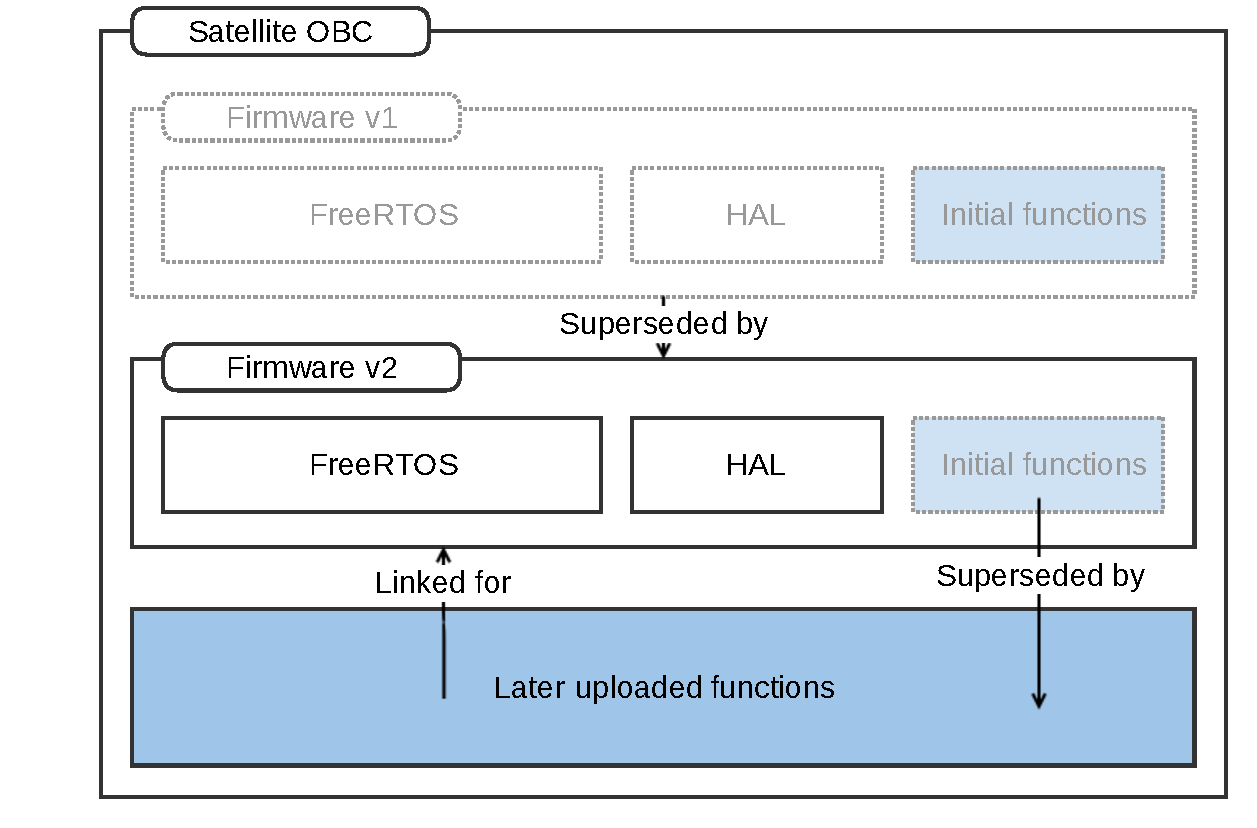
\includegraphics[width=0.9\textwidth]{figures/On-board_software_organization.pdf}
	\caption{Proposed on-board software organization. Blue denotes application software.}
	\label{fig:swOrg}
\end{figure}

% divided by function
Application software, on the other hand, would be divided into parts, each containing a single function. Each application function would be combined with a short header (Table~\ref{tab:header}) to form a package. Each function could then be independently updated, added or removed.

\begin{table}[ht]
	\centering
	\caption{Application function's header.}
	\begin{tabular}{r|l|l}
		\bf{Length (bytes)} & \bf{Field} & \bf{Format} \\
		\hline
		4 & \Gls{crc} & CRC-32 \\
		\hline
		1 & Type &
		\begin{tabular}{r|l}
			\texttt{0xff} & nothing \\
			\texttt{0xaa} & function \\
			\texttt{0x55} & global \\
			\texttt{0x00} & disabled \\
		\end{tabular} \\
		\hline
		2 & Function ID & uint16 \\
		\hline
		1 & Version no & uint8 \\
		\hline
		2 & Length of body & uint16 \\
		\hline
		2 & \Gls{sram} offset (global variables only) & uint16 \\
	\end{tabular}
	\label{tab:header}
\end{table}

% padding
The headers (Table~\ref{tab:header}) will have \texttt{nop}-instructions appended to them to pad them to 12 bytes in length. Some instructions will generate a fault or will execute slower if addresses are not word-aligned \cite[Section~3.3.5]{STMicroelectronics2017}, therefore a multiple of 4 bytes was chosen for the header length.

% snapshots
Function version dependencies would be managed by a system of snapshots similar to git \cite[Chapter~1.3]{Chacon2018}: after new functionality has been developed and tested, current version of all functions is recorded. \Gls{mcs} will then determine, which of them differ when compared to satellite's internal storage, and upload those.

\subsubsection{On-board storage of application software}

Main focus is on storing application functions in internal flash, since it is the most restrictive storage. Additionally, in safe mode, this is the sole non-volatile storage available (Section~\ref{s:hardware}). Storage of some functions in other memories, as well as moving functions between different memories and addresses, would also be possible.

While flash memory does not support deleting or changing any data short of an entire sector, new data can be appended. Functions would therefore be written to flash sequentially as they arrive. Additionally, flash allows the addition of zeros into data. This way functions could be marked as disabled by replacing some predefined area of function header with zeros ('Type' in Table~\ref{tab:header}), without the need to delete the sector. In order to change a function, a new version would simply be appended to the storage. If several versions of a function are found in memory, the last one will be considered correct.

\subsubsection{Linking}

Compiled code contains many symbol references: function calls, global variables, etc. For software to run, all of them must be replaced with absolute memory addresses. In order to satisfy all requirements (especially about no modifications to uploaded code), a combination of static pre-linking and custom dynamic linker would be used.

Firmware would be compiled and linked to a fixed memory address first - meaning that absolute memory addresses of all functions and global variables in the firmware would be fixed. This way calls to all firmware functions from other firmware functions, as well as from any later added application functions, can be simply linked on the ground (Figure~\ref{fig:swLink}).

\begin{figure}[ht]
	\centering
	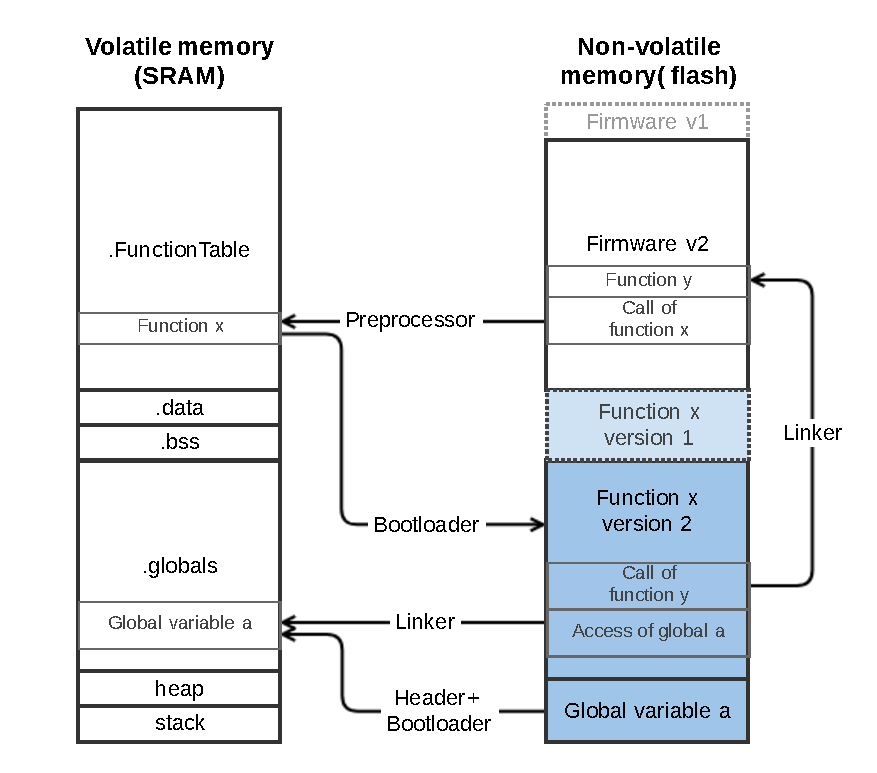
\includegraphics[width=0.96\textwidth]{figures/Software_linking.pdf}
	\caption{References in on-board software. Blue denotes application software.}
	\label{fig:swLink}
\end{figure}

Calling application functions is more tricky, as they can move around in memory. They would be callable by using a system-global offset table (Figure~\ref{fig:swLink}). This table would contain the current memory address for each function. It will be stored in volatile internal \gls{sram} and re-created every time the system boots (by walking over all stored functions and storing the address where each function appears last). The table itself would be located on fixed memory location and contain functions sorted by id. It can be also changed during the run-time, when new functions are added. Changing it during the run-time when a function is changed requires additional checks to guarantee that previous memory address does not remain in use (as some function pointer somewhere) and is therefore out of the scope of this work, but is a potential future improvement.

Additionally, firmware can't call functions, whose signatures are not known at the time of firmware compilation, since compiler must generate code for passing arguments. For that reason, some functions are bundled with the firmware (Figure~\ref{fig:swOrg}). Examples would include functions dealing with the \gls{icp} and software updating itself. They can be updated, but their signatures must remain unchanged.

The table of function offsets would be periodically checked for errors. Functions' checksums could also be checked during the generation of this table. During reboot, flash memory can also be defragmented.

\subsubsection{Compiling application functions}

Compilers support generating indirect function calls out of the box for \gls{pic}. However, the commonly-used \gls{svr4} scheme expects the \gls{got} to be at a fixed offset from the code \cite[Chapter~8]{Levine1999}. This has the effect that each independent portion of code needs its own copy of the \gls{got}, but having one for each function would cause unacceptable size overhead. To avoid having to modify the compiler itself, a way to rewrite all function calls using the preprocessor will be used.

For each function that would otherwise result in an unresolved external symbol, a preprocessor macro (Figure~\ref{fig:macro}) will be generated. It contains instructions to read function's address from the function table, cast it to the function's type, cast all arguments to required types, and call the function. Since the macro call syntax will be identical to that of a function call, application code can be agnostic to the updating platform.

\begin{figure} [htb]
\begin{lstlisting}[language=C]
typedef void (*f0_t)();
#define f0() (*((f0_t)(*((uint32_t *) (0x20000000)))))()
\end{lstlisting}
\caption{Call interception macro for the hypothetical function \texttt{f0()} with id 0, where the function table is located at a fixed address \texttt{0x20000000}.}
\label{fig:macro}
\end{figure}

For calling important functions, the checksum of the function can be checked immediately before jumping by incorporating modified interception macro. Normally this is not done.

\subsubsection{Global variables}

In order to simplify the design, global variables would be treated very similarly to functions. First, they would be compiled, since then the the compiler would calculate their lengths. Compilation should include the flag \texttt{-fdata-sections}, this way they can be extracted to separate packages, prepended with headers, and uploaded to the satellite.

Memory space after \texttt{.data} and before heap would be reserved for updatable global variables  (Figure~\ref{fig:swLink}). Linker would select an address for each variable in that area, and then all functions using the variable could be statically pre-linked on the ground. Headers for global variables would contain the appropriate type, and additionally the memory address allocated for this variable (Table~\ref{tab:header}). During boot, when function addresses are being added to the offset table, global variables would be copied to their respective addresses (Appendix~\ref{apx:gentable}). As with a function, the latest occurrence of a global variable overrides any previous ones.

\clearpage
\section{Conclusion}
\label{s:conclusion}

In this paper

\TODO{what did you do?}
\TODO{What are the results?}
\TODO{saavutatu põhjendatud ja ammendav võrdlus varasemate tulemustega}
\TODO{tulemuste rakendatavus}
\TODO{future work?}



% BibTeX bibliography
\newpage
\nocite{*}
\TODO{Remove nocite}
%\bibliography{bachelor-thesis}
\printbibliography
\addcontentsline{toc}{section}{\refname}

% All extras and licence:
\newpage
%\appendix
%\iflanguage{english}%
%  {\section{Appendix}
%  \addcontentsline{toc}{section}{Appendix}
%  }%
%  {\section{Lisad}
%  \addcontentsline{toc}{section}{Lisad}}

%\subsection{Glossary}
%\addcontentsline{toc}{subsection}{I. Glossary}
\begin{appendices}
\printglossaries

\newpage
\section{Indirect function calls}
\label{apx:calls}
\begin{lstlisting}[style=asm]
// Experiment to quantify the exact memory/speed tradeoff when using 24 vs 32 bits per function pointer in function table
// Decision: 32 bits makes more sense in this case
.syntax unified
.cpu cortex-m7
.thumb

function: // Function to be called
bx lr // Immideately return

jump32: // How would function call overhead look like in case of 32 bits of RAM per function pointer
ldr r0, [r1]
bx r0

jump24: // How would function call overhead look like in case of 24 bits of RAM per function pointer
ldr r0, [r1]
lsr r0, r0, #8
orr r0, 0x08000000
bx r0

.type  Reset_Handler, %function
Reset_Handler:
ldr sp, =_estack
ldr r1, =function // Load function pointer into register 1
bl jump32
sub r1, #1 // Subtract one byte from the label address because 24 bits have to be right-aligned
bl jump24
loop:
b loop

.section  .isr_vector,"a" // Interrupt Service Routines vector table, "a"llocatable
g_pfnVectors:
.word _estack // End of stack; defined in linkerscript
.word Reset_Handler
\end{lstlisting}


\newpage
\section{Boot sequence}
\label{apx:gentable}
\begin{lstlisting}[language=C]
volatile uint32_t __attribute__((section(".FunctionTable"))) FunctionTable[255];

void gentable(uint32_t *start) {
	uint8_t *bytestart = (uint8_t *)start;
	while (1) {
		uint32_t *crc        = (uint32_t *)(bytestart     );
		uint8_t  *type       = (uint8_t  *)(bytestart +  4);
		uint16_t *id         = (uint16_t *)(bytestart +  5);
		uint8_t  *version    = (uint8_t  *)(bytestart +  7);
		uint16_t *length     = (uint16_t *)(bytestart +  8);
		uint16_t *vma_offset = (uint16_t *)(bytestart + 10);
		
		if (*type == 0b10101010) {
			FunctionTable[*id] = (uint32_t)bytestart+12+1;
			bytestart += 12 + *length;
		} else if (*type == 0b01010101) {
			memcpy((void*)(0x20000000 + *vma_offset), bytestart, *length);
			bytestart += 12 + *length;
		} else if (*type == 0b11111111) {
			break;
		} else if (*type == 0b00000000) {
			bytestart += 12 + *length;
		}
	}
}
\end{lstlisting}

\newpage
%=== Licence in English
\newcommand\EngLicence{{%
\selectlanguage{english}
\section{Licence}

%\addcontentsline{toc}{subsection}{II. Licence}

\subsection*{Non-exclusive licence to reproduce thesis and make thesis public}

I, \textbf{\Author},

\begin{enumerate}
\item
herewith grant the University of Tartu a free permit (non-exclusive licence) to:
\begin{enumerate}
\item[1.1]
reproduce, for the purpose of preservation and making available to the public, including for addition to the DSpace digital archives until expiry of the term of validity of the copyright, and
\item[1.2]
make available to the public via the web environment of the University of Tartu, including via the DSpace digital archives until expiry of the term of validity of the copyright,
\end{enumerate}

of my thesis

\textbf{\topic}

supervised by \SupervisorName\ and \CosupervisorName.

\item
I am aware of the fact that the author retains these rights.
\item
I certify that granting the non-exclusive licence does not infringe the intellectual property rights or rights arising from the Personal Data Protection Act. 
\end{enumerate}


Tartu, \today
}}%\newcommand\EngLicence


%=== Licence in Estonian
\newcommand\EstLicence{{%
\selectlanguage{estonian}
\section*{II. Litsents}

\addcontentsline{toc}{subsection}{II. Litsents}

\subsection*{\topic}

Mina, \textbf{\Author},

\begin{enumerate}
\item
annan Tartu Ülikoolile tasuta loa (lihtlitsentsi) enda loodud teose

\textbf{\topic}

mille juhendajad on \JuhendajaName\ ja \KaasjuhendajaName

\begin{enumerate}
\item[1.1]
reprodutseerimiseks säilitamise ja üldsusele kättesaadavaks tegemise eesmärgil, sealhulgas digitaalarhiivi DSpace-is lisamise eesmärgil kuni autoriõiguse kehtivuse tähtaja lõppemiseni;
\item[1.2]
üldsusele kättesaadavaks tegemiseks Tartu Ülikooli veebikeskkonna kaudu, sealhulgas digitaalarhiivi DSpace´i kaudu kuni autoriõiguse kehtivuse tähtaja lõppemiseni.
\end{enumerate}


\item
olen teadlik, et punktis 1 nimetatud õigused jäävad alles ka autorile.
\item
kinnitan, et lihtlitsentsi andmisega ei rikuta teiste isikute intellektuaalomandi ega isikuandmete kaitse seadusest tulenevaid õigusi. 
\end{enumerate}


Tartus, \today
}}%\newcommand\EstLicence


%===Choose the licence in active language
\iflanguage{english}{\EngLicence}{\EstLicence}

\end{appendices}

\end{document}

